\section{Qsim::VmQItem Struct Reference}
\label{structQsim_1_1VmQItem}\index{Qsim::VmQItem@{Qsim::VmQItem}}
{\tt \#include $<$qsim.h$>$}

Inheritance diagram for Qsim::VmQItem:\nopagebreak
\begin{figure}[H]
\begin{center}
\leavevmode
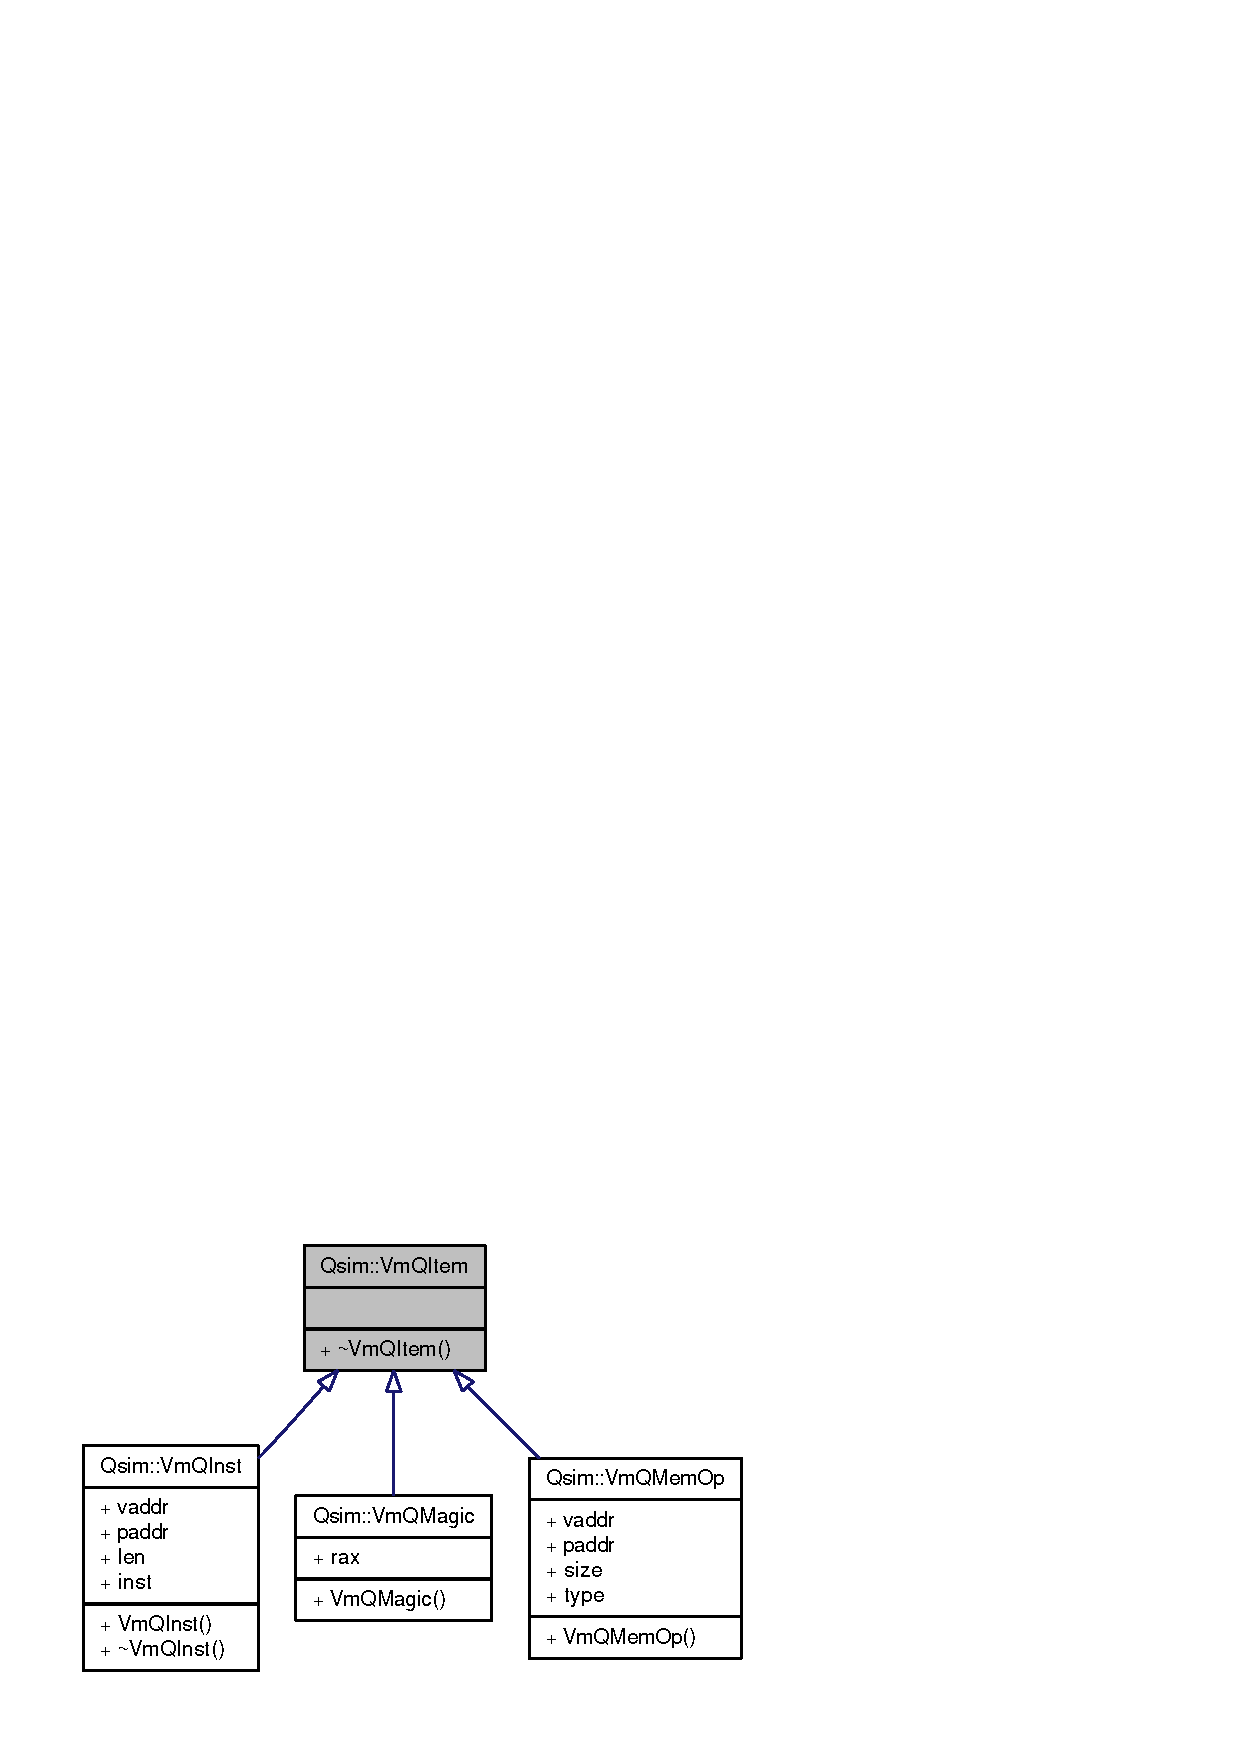
\includegraphics[width=360pt]{structQsim_1_1VmQItem__inherit__graph}
\end{center}
\end{figure}
\subsection*{Public Member Functions}
\begin{CompactItemize}
\item 
virtual {\bf $\sim$VmQItem} ()
\end{CompactItemize}


\subsection{Detailed Description}


Definition at line 90 of file qsim.h.

\subsection{Constructor \& Destructor Documentation}
\index{Qsim::VmQItem@{Qsim::VmQItem}!$\sim$VmQItem@{$\sim$VmQItem}}
\index{$\sim$VmQItem@{$\sim$VmQItem}!Qsim::VmQItem@{Qsim::VmQItem}}
\subsubsection[{$\sim$VmQItem}]{\setlength{\rightskip}{0pt plus 5cm}virtual Qsim::VmQItem::$\sim$VmQItem ()\hspace{0.3cm}{\tt  [inline, virtual]}}\label{structQsim_1_1VmQItem_8a88fbb4e7fdff1866eb67a373d0d43e}




Definition at line 90 of file qsim.h.

References $\sim$VmQItem().

Referenced by $\sim$VmQItem().

Here is the caller graph for this function:\nopagebreak
\begin{figure}[H]
\begin{center}
\leavevmode
\includegraphics[width=93pt]{structQsim_1_1VmQItem_8a88fbb4e7fdff1866eb67a373d0d43e_icgraph}
\end{center}
\end{figure}


The documentation for this struct was generated from the following file:\begin{CompactItemize}
\item 
{\bf qsim.h}\end{CompactItemize}
